
\section{Class Diagram}
\subsection{Architecture Overview}
Our system's architecture employs a foursome design pattern, dividing the application into four main layers: the AI backend, the backend, the database, and the frontend. Each layer has distinct responsibilities and interacts with other layers to ensure seamless functionality.

\newpage 

\subsection{Class Diagrams}
\subsubsection{Overall Architecture}
\begin{figure}[h]
  \centering
  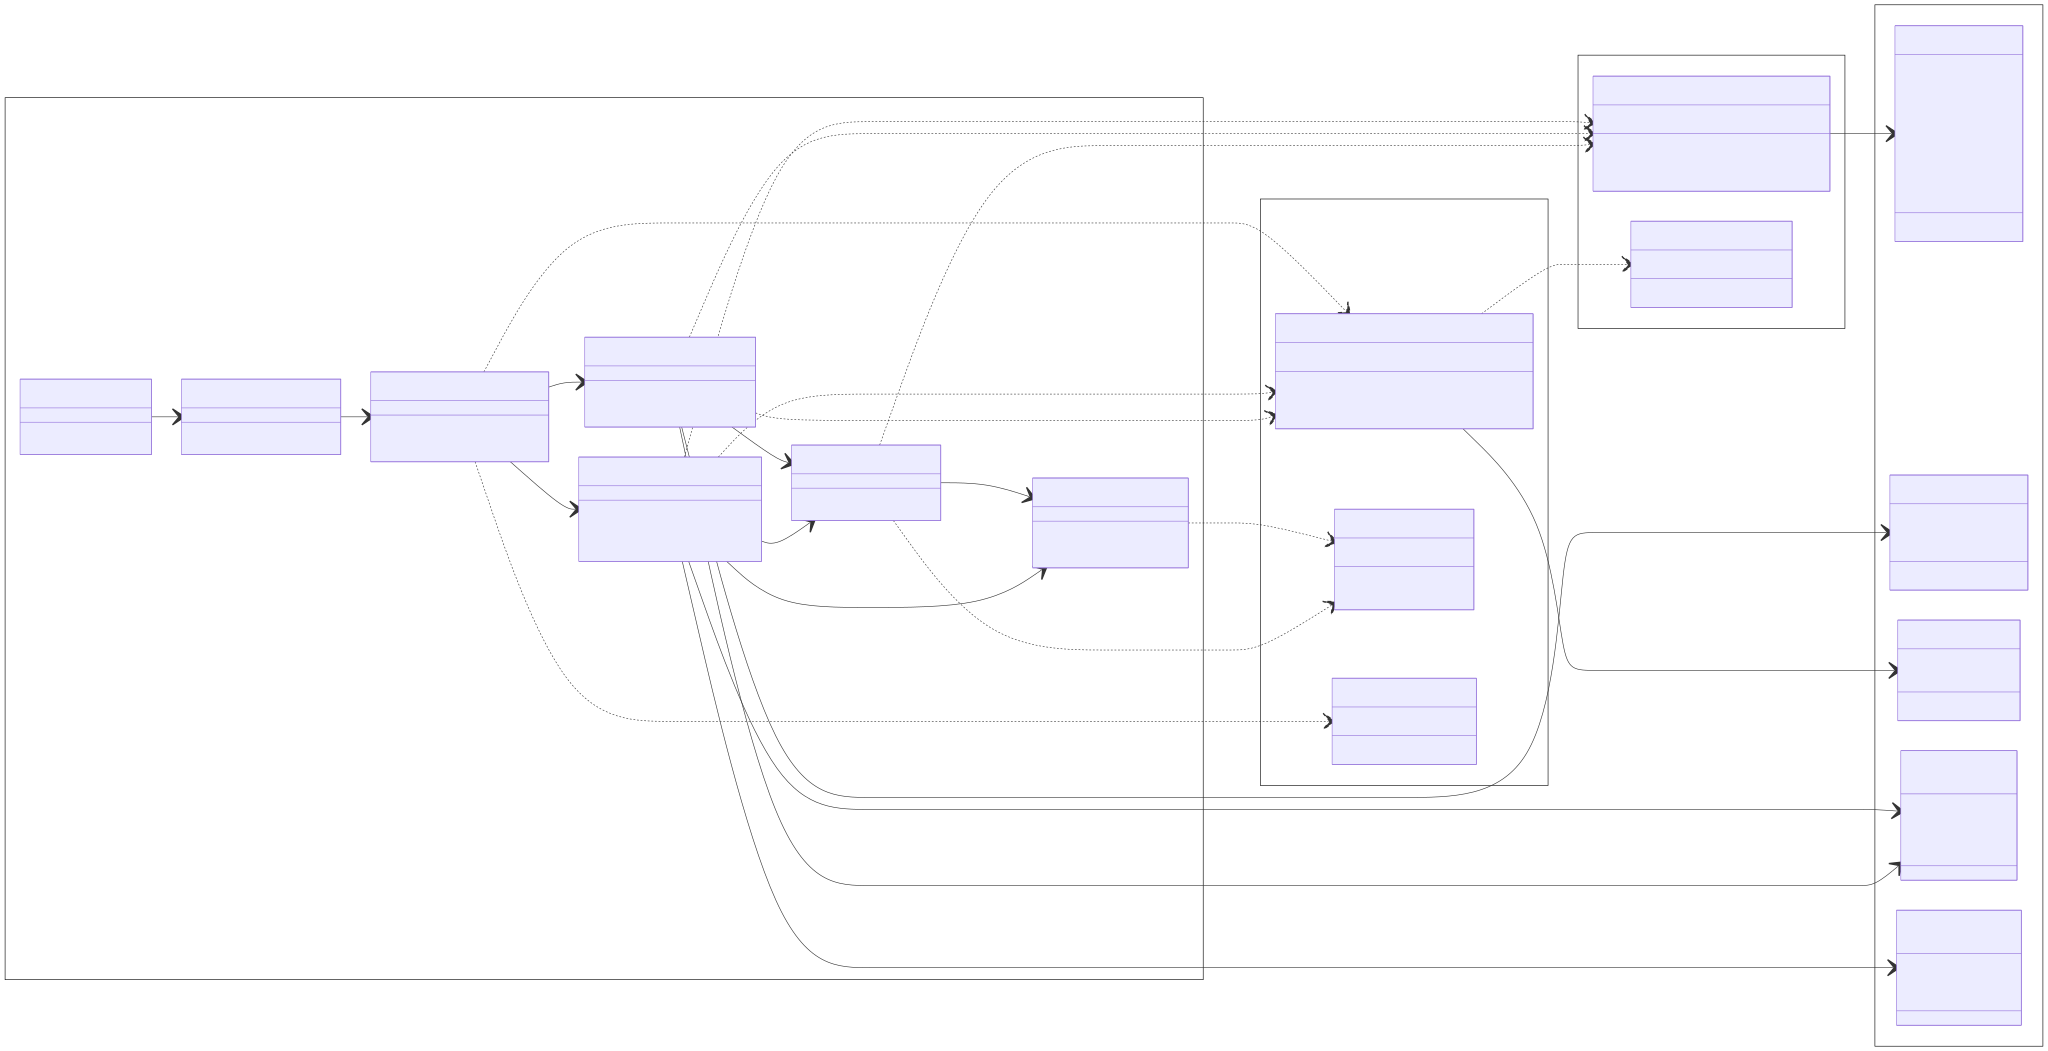
\includegraphics[width=\linewidth]{uml/class-diagram.svg}
  \caption{Overall architecture.}
\end{figure}

\quad The class diagram above illustrates the overall architecture of the system. It shows a Flutter frontend with UI screens (MyApp, IntroductionScreen, HomeScreen, SearchScreen, RegionOverview, PlaceOverview, MapScreen) connected by navigation edges. State is managed via Riverpod providers: UserSessionProvider (user state and preferences), SelectedPlaceProvider (current place), and NavigationIndexProvider (current tab). Service layer classes (PlaceService, ProfileService) wrap Dio HTTP calls to fetch places (by query, ID, or image) and user profiles. Models include Place, Region, User, and enum types FilterType and CategoryType. Screens read or set provider state: Home/Search/Region read UserSession; PlaceOverview sets SelectedPlace; MapScreen listens to SelectedPlace; Home sets NavigationIndex. Services supply data to UI and providers, and models represent the domain entities and filters used across the app.
\newpage

\subsubsection{AI Backend, Backend, and Database}                                                                                                                                                       
\begin{figure}[h]
  \centering
  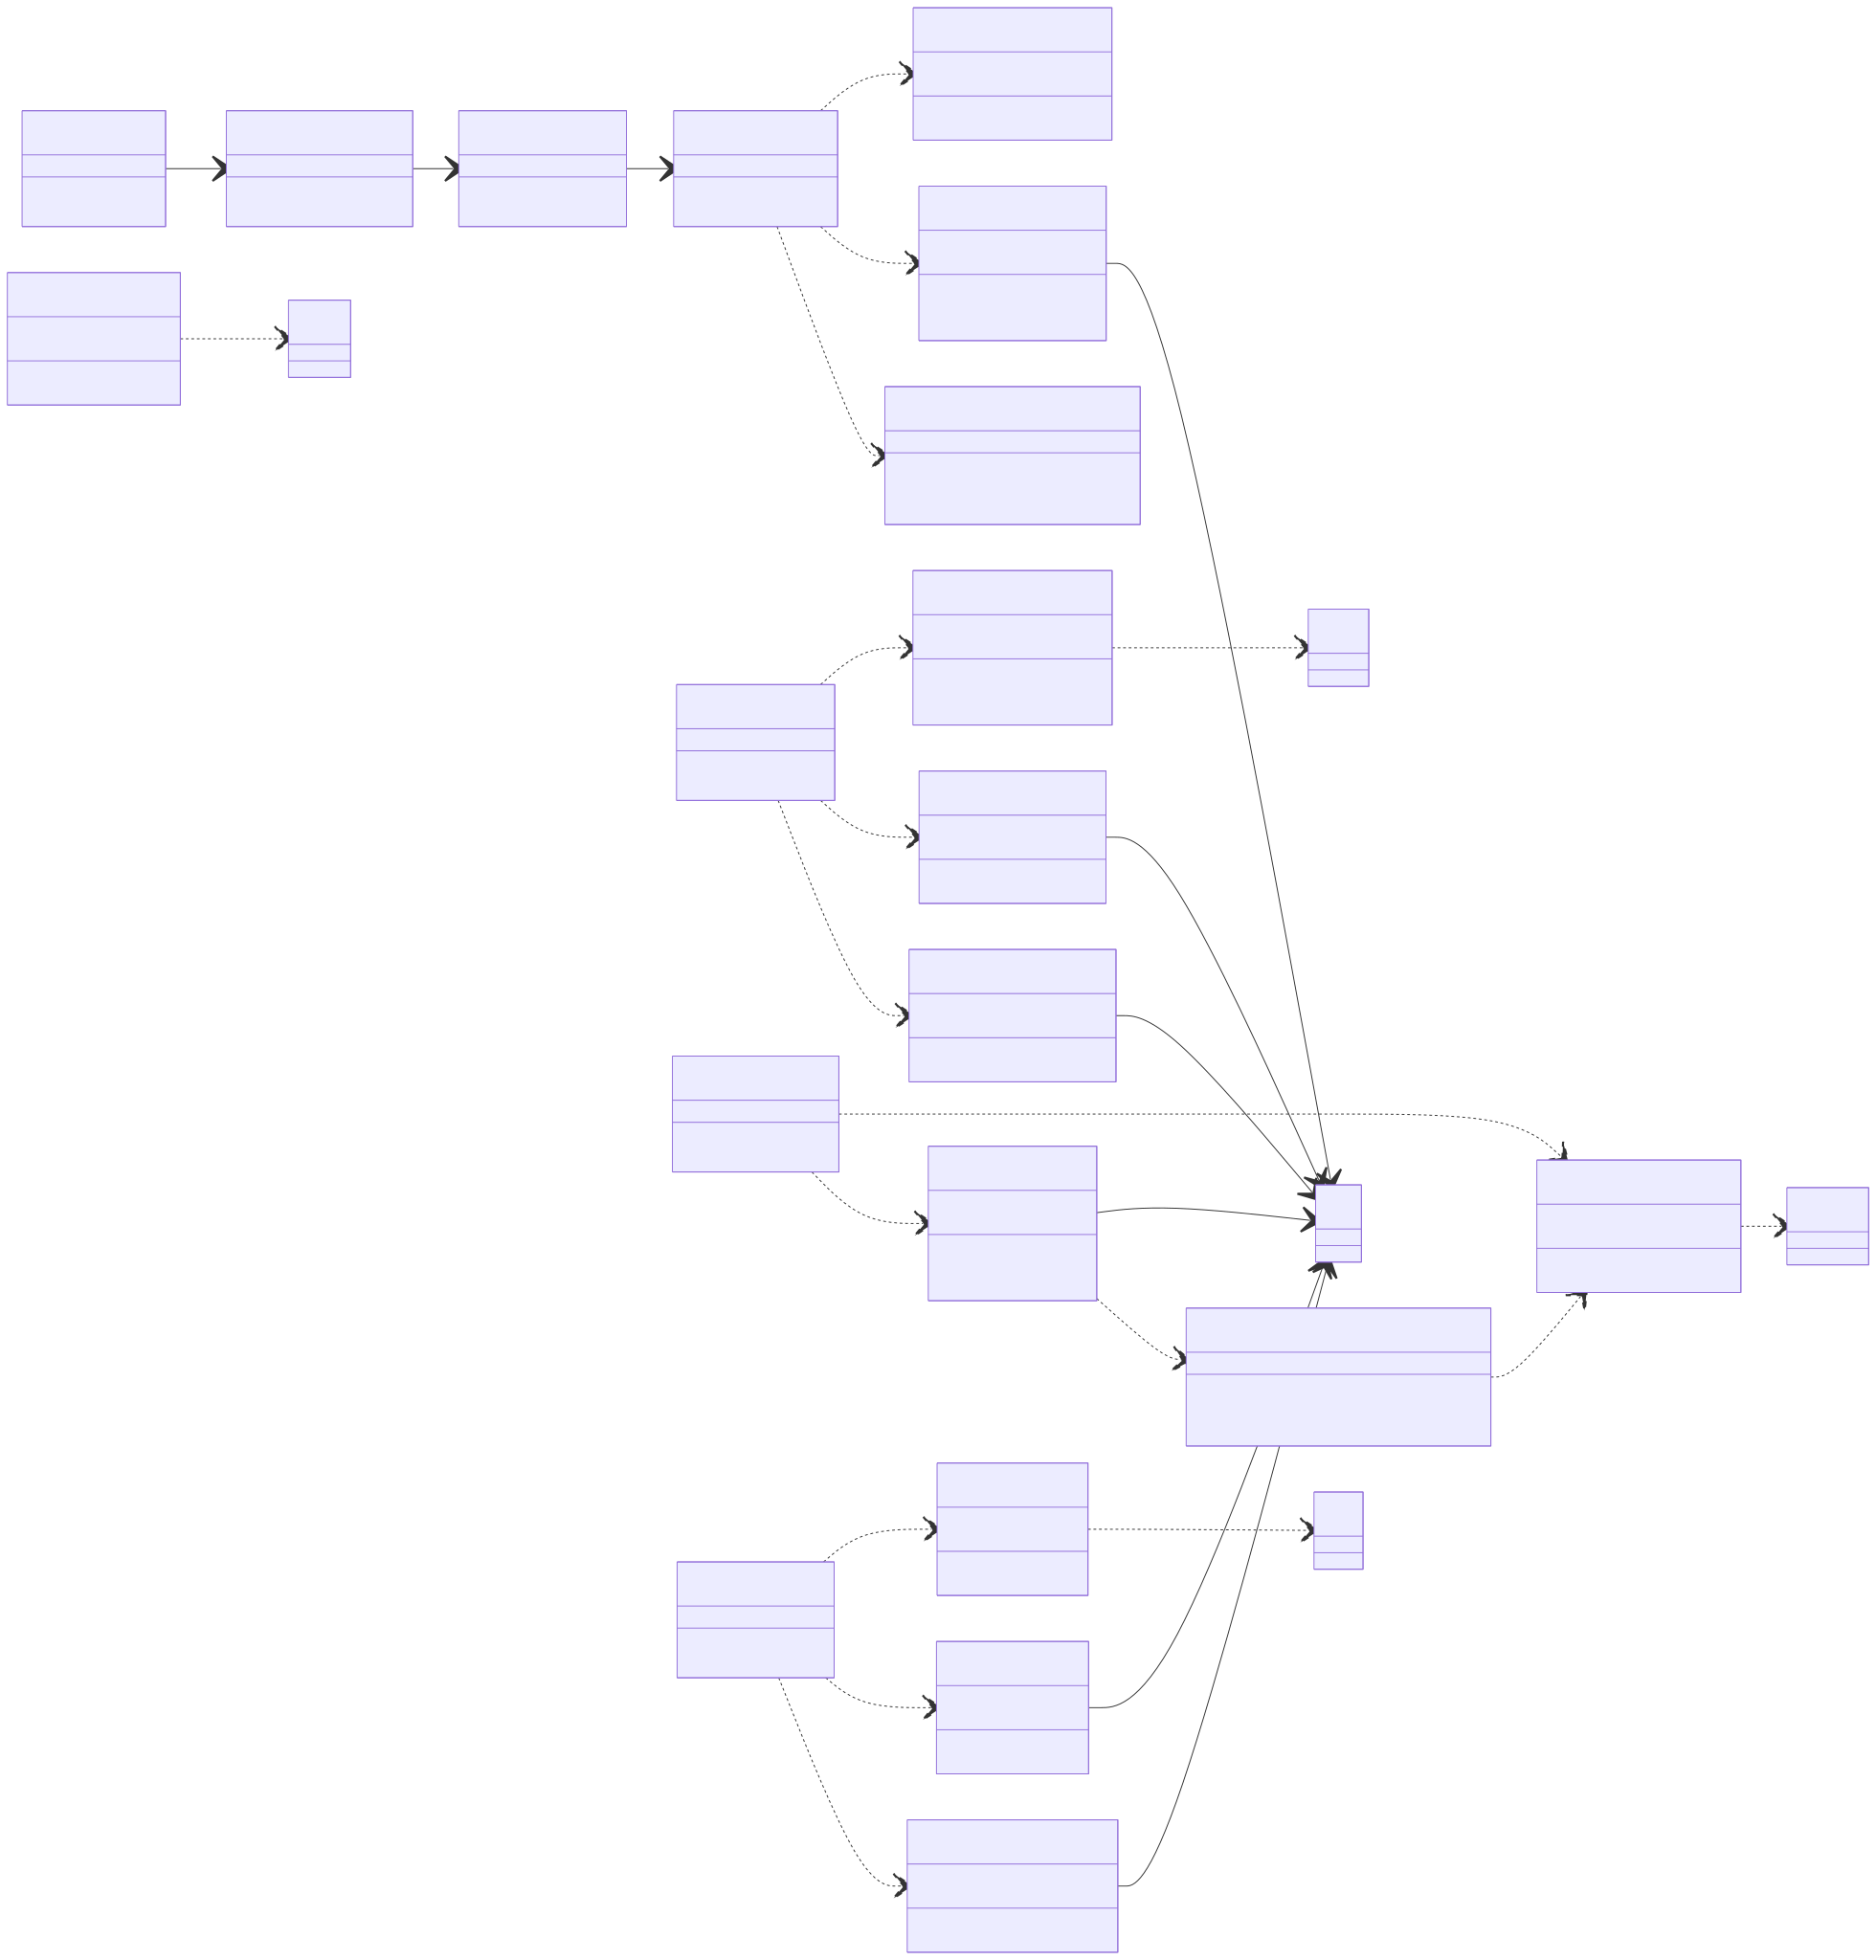
\includegraphics[width=\linewidth]{uml/class-diagram-frontend.svg}
  \caption{Frontend architecture.}
\end{figure}

\quad The Flutter frontend boots via `MyApp`, routing first to `IntroductionScreen` and then into the main flow (Splash, Home, Map, Profile, Trip). UI screens read Riverpod providers for navigation (`NavigationProvider`), selection (`SelectedPlaceProvider`), user/session (`UserInfoProvider`), trips (`TripProvider`), and events. Screens invoke service classes for API calls: `PlaceService`, `EventService`, `GeocodeService`, `MapService`, `ReviewService`, and `AuthService`, with `SearchCacheService` caching queries locally. All HTTP calls share a Dio client; `ServiceHelpers` centralizes error handling and token refresh before updating session state through providers.

\newpage
\begin{figure}[h]
  \centering
  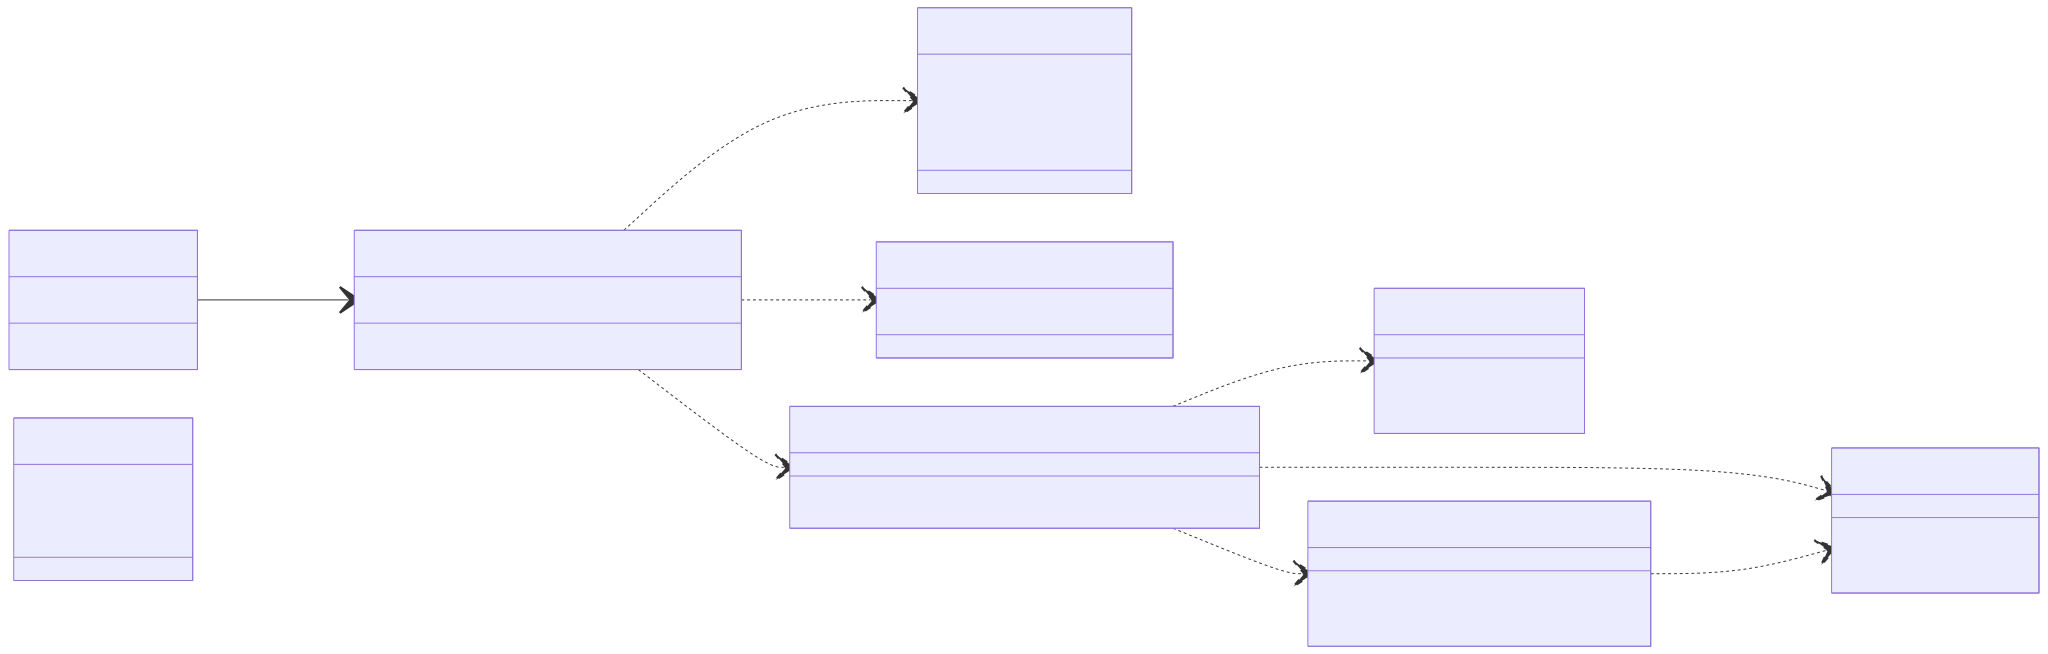
\includegraphics[width=\linewidth]{uml/class-diagram-ai-backend.svg}
  \caption{AI backend architecture.}
\end{figure}

\quad The ai_backend is a FastAPI app that exposes a recommendation endpoint. The entrypoint (Main) creates the FastAPI app, adds CORS middleware, and includes the RecommendationRouter. The router defines the recommend(...) endpoint, which accepts a RecommendationRequest (user_id, query, top_k, filters) and returns a RecommendationResponse containing a list of ItemScore (place_id, score, explanation).

\newpage

\begin{figure}[h]
  \centering
  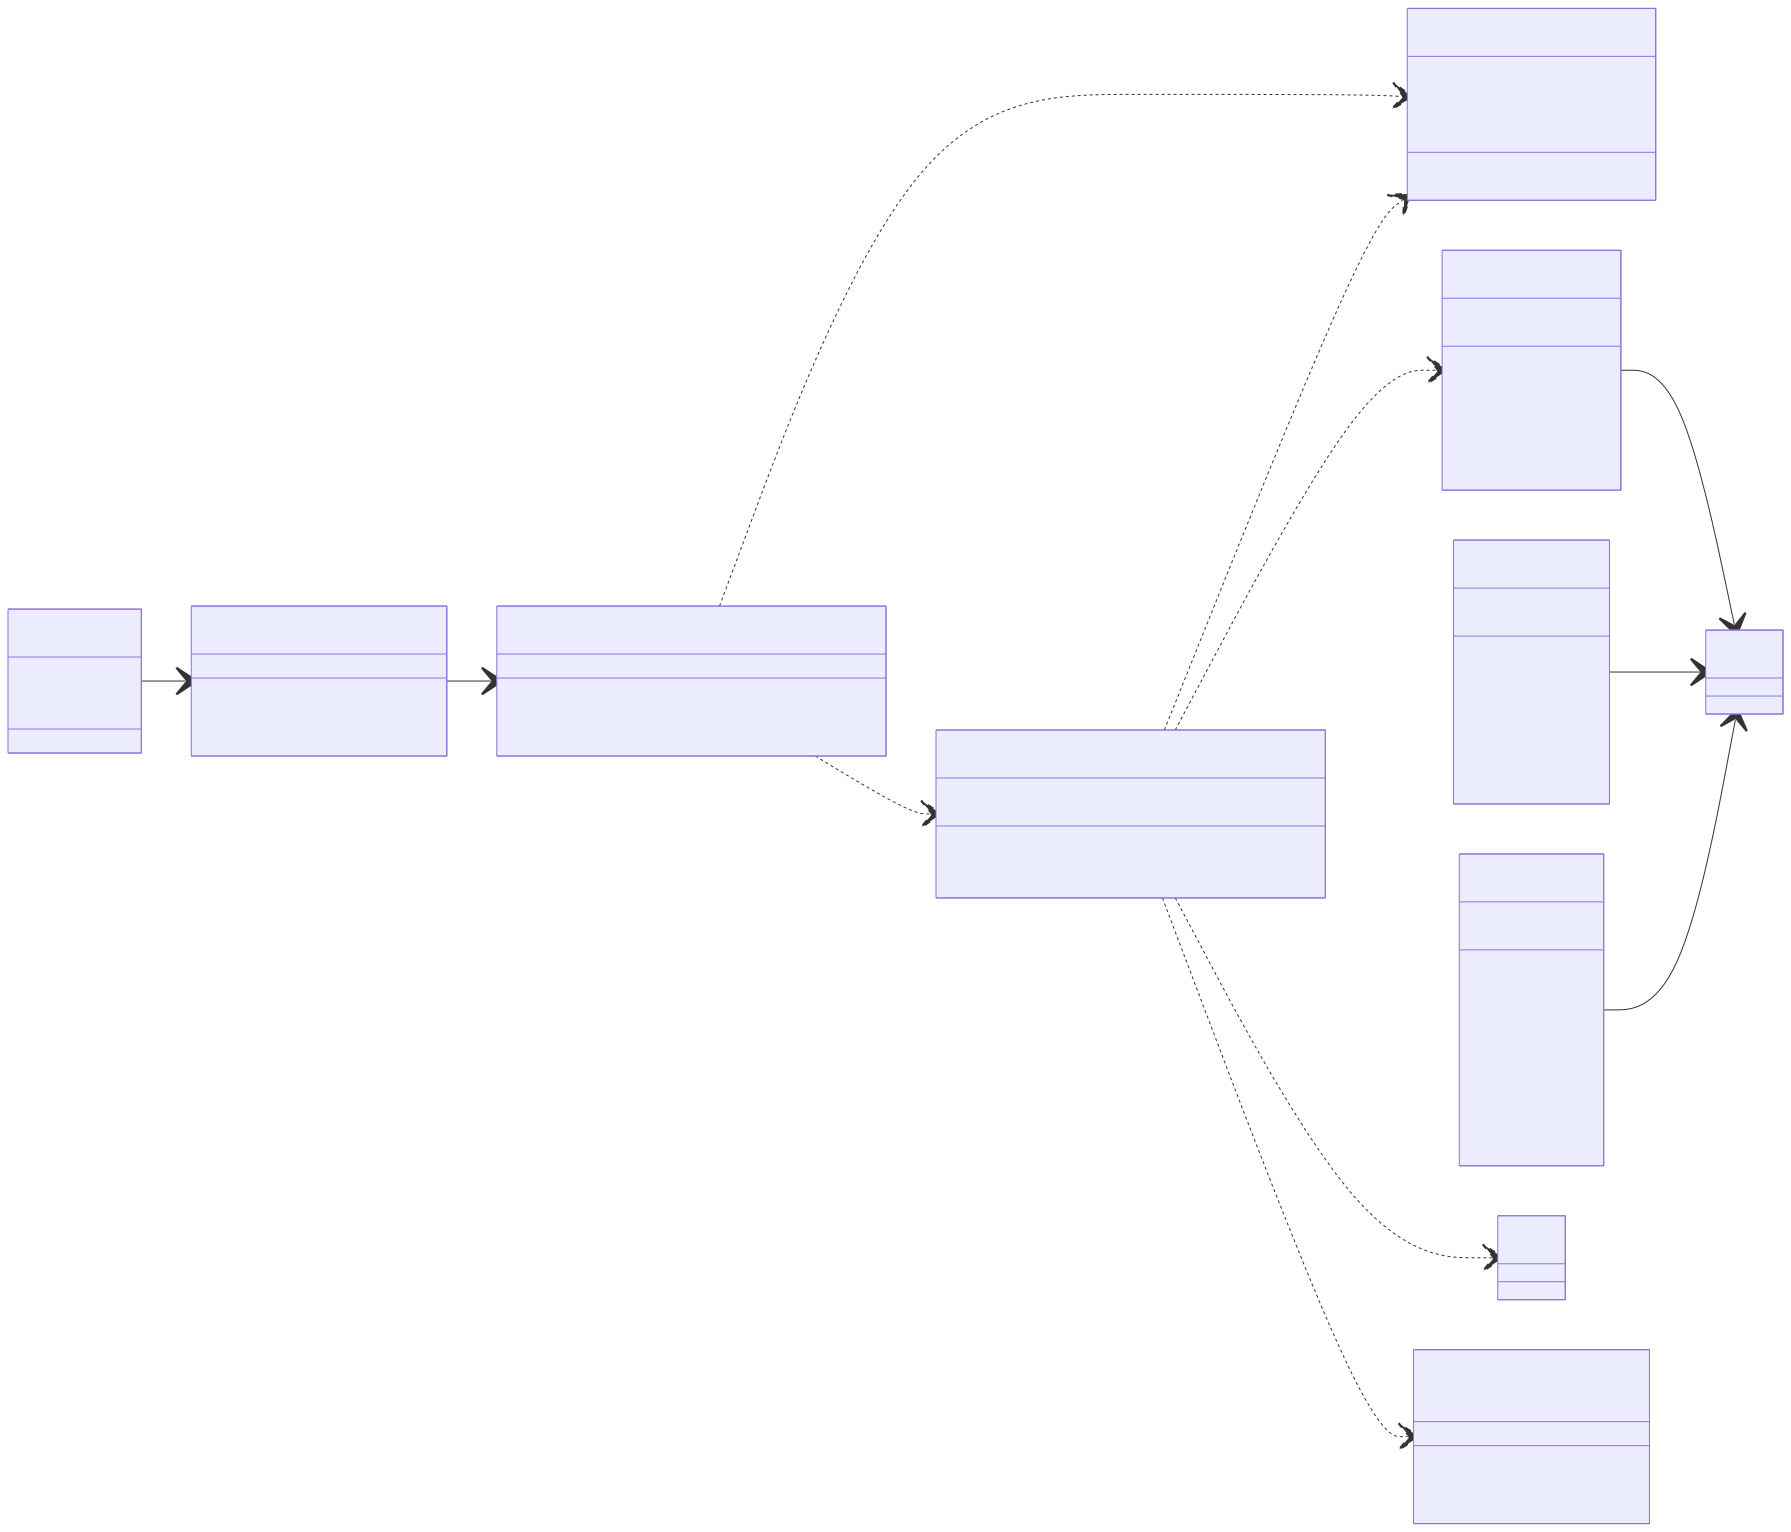
\includegraphics[width=\linewidth]{uml/class-diagram-backend.svg}
  \caption{Backend architecture.}
\end{figure}

\quad The backend is an Express app that wires routes to controllers and services. The entry `App` holds the Express instance and registers `RecommendationRoutes`, which map HTTP handlers to `RecommendationController`. Controllers delegate to `RecommendationService` to call the Python AI backend via Axios and wrap responses in `ServiceResponse`. Enmap-backed stores (`UserDB`, `LocationDB`, `EventDB`) provide simple persistence layers for user state, geocoded locations, and events. `RecommendationService` depends on these stores to enrich requests and cache results, while also calling the external `PythonRecAPI` for recommendations and feedback.

\begin{figure}[h]
  \centering
  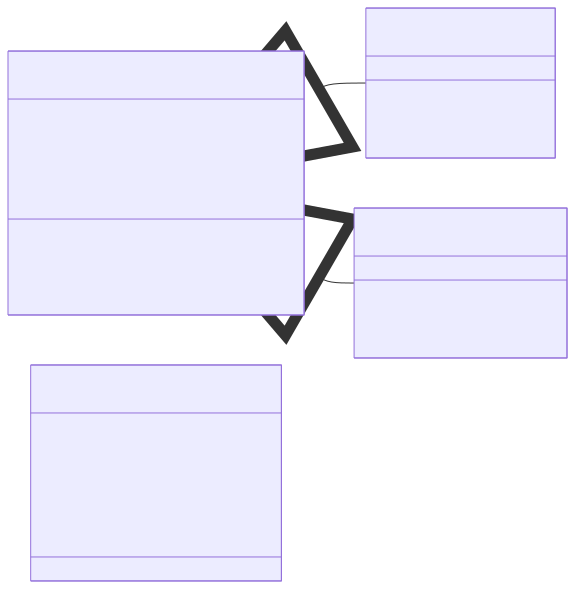
\includegraphics[width=\linewidth]{uml/class-diagram-db.svg}
  \caption{Database architecture.}
\end{figure}

\quad The data layer loads CSVs into DataFrames, builds text+metadata docs, and keeps stable IDs (geo keys or MD5 fallback). BaseColInfo centralizes this; ArchColInfo and RestaurantColInfo tailor narratives for architecture and food. Outputs feed ChromaDB (vector) and BM25 (keyword) search, fused and reranked before the FastAPI /search endpoint returns scored items.
